\documentclass[documentation.tex]{subfiles}
\begin{document}
    Ще разгледаме проблемите, които решава библиотеката от три гледни точки:
    \subsection{Ученици}
    \begin{text} \par
        В повечето профилирани училища учениците се сблъскват с прогромният език С++, който се е наложил като лесноусвойм от тийнейджърите.
    \end{text} \\
    \begin{text} \par
        На фона на всичко позитивно учениците не виждат приложната страна на езика, който се е наложил като един от най-ефективните (ако не и най-ефективният) за разработка на игри.
    \end{text}
    \begin{text} \par
        Проведох непредставително проучване сред ученици от 10. и 11. клас на Софийската математическа гимназия.\cite{form} Ето и резултатите от него:\\
    \end{text}
    \begin{center}
        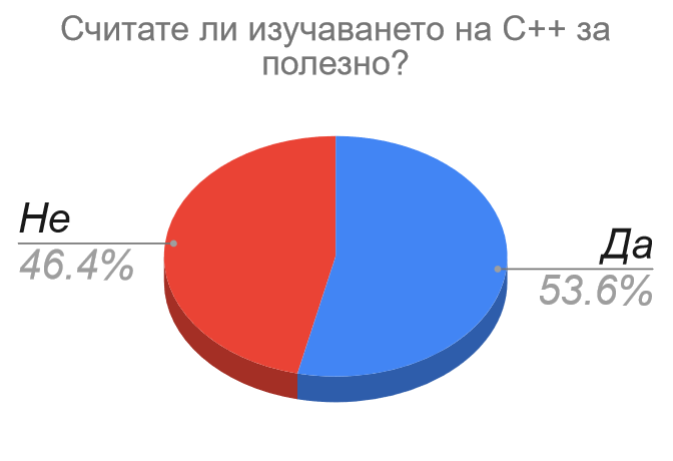
\includegraphics[width=0.75\textwidth]{images/learning.png}\\
        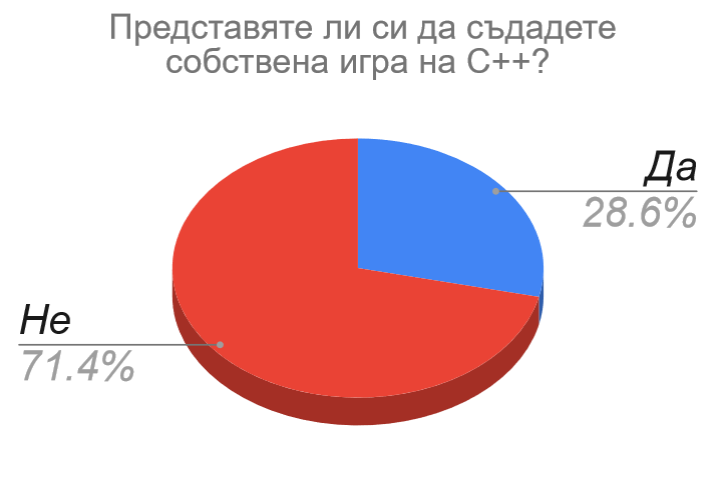
\includegraphics[width=0.75\textwidth]{images/games.png}\\
        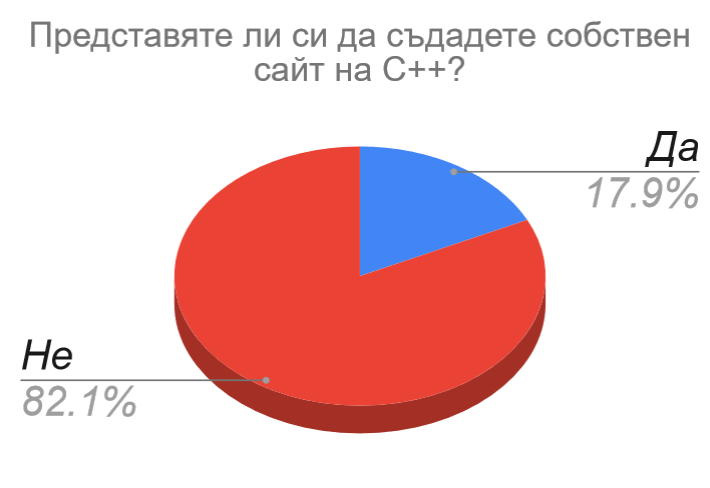
\includegraphics[width=0.75\textwidth]{images/web.png}\\
    \end{center}
    \begin{text} \par
        От тази гледна точка създаването на първия си сайт в училище със знания от час значително повишава интереса към учебния процес.
    \end{text}
    \subsection{Състезатели}
    \begin{text} \par
        По националните състезания по информатика се забелязва тенденция на демотивация на участниците с тенденциозно място извън челните. Те вече знаят програмният език достатъчно добре и библиотеката ще им позволи бързо да пренасочат знанията си към приложната сфера, където състезателите могат да са на челните места, впечатлявайки със скоростта на продукта си. (\ref{compare}) На фона на всичко времето, което ще е необходимо за „преориентиране“ към библиотеката, е минимално.
    \end{text}
    \subsection{Бизнеса}
    \begin{text} \par
        Благодарение на интерфейса на библиотеката, бизнесът може много бързо да мигрира към нея. Използването ѝ ще допринесе за разрастването на компанията поради наличието на ученици със знания за технологията - т.е. повече квалифицирана работна ръка.
    \end{text}
    
\end{document}

